\subsubsection{Mobiiliverkko}
\begin{figure}[htb]
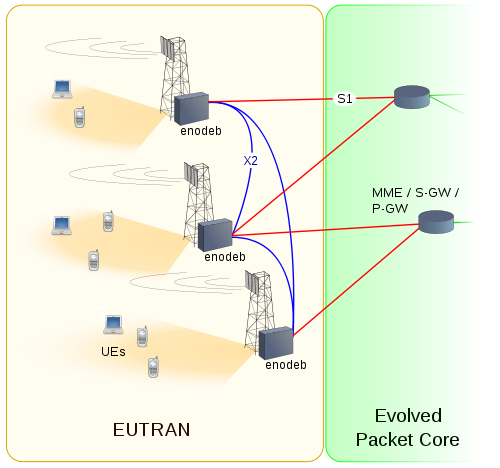
\includegraphics[scale=0.5]{EUTRAN}
\caption{Mobiiliverkon rakenne} \label{ekakuva}
\end{figure}

MEC ehdotuksia tarkasteltaessa, olemassa olevien mobiiliverkkojen arkkitehtuurit ovat keskeisessä asemassa. Useat reunalaskentaa käsittelevät ehdotukset on tarkoitettu integroitaviksi osaksi olemassa olevaa mobiiliverkkoarkkitehtuuria. 
Erityisesti asiakaslaitteiden ollessa mobiililaitteita ja mahdollisimman pieniä viiveitä tavoiteltaessa, reunalaskenta ratkaisujen integroiminen osaksi mobiiliverkkoa on väistämätöntä. Seuraavaksi käydään pääpiirteittäin läpi 4G mobiiliverkon arkkitehtuurin funktionaaliset osat.

Yksinkertaistettuna mobiiliverkko koostuu kahdesta osasta: radiorajapinnasta ja mobiilinverkon runkoverkosta (puhelinkeskuksesta?). 3GPP kehittämässä LTE standardissa radiorajapinnan sisältävä osuus on nimeltään E-UTRAN (Evolved UMTS Terrestrial Radio Access Network) ja runkoverkon osuus EPC (Evolved Packet Core).

E-UTRAN tehtävänä on toimia rajapintana asiakaslaitteen ja EPC:n välillä. Asiakaslaitteiden suuntaan yhteys on radiosignalointia ja yhtenä E-UTRAN tehtävänä onkin radioresurssien hallinointi. 
E-UTRAN sisältää verkon puolella pääasiallisena toimijana eNodeB tyyppisiä tukiasemia \cite{etsieutran}, myös muutamia poikkeustapauksia on, mutta ne jätetään käsittelemättä.
Tukiasema on asiakaslaitetta lähimpänä sijaitseva funktionaalinen verkon osa ja sen seurauksena se on houkutteleva kohde MEC ratkaisuille. Tukiasemaa voikin ajatella \textit{reunan} viimeisenä etappina ennen asiakaslaitetta. Tämä tutkielma käsittelee pääasiassa ratkaisuja, jotka keskittyvät LTE verkkoihin kohdistuvia ratkaisuja, joten tukiasemista puhuttaessa tarkoitetaan nimenomaan E-UTRAN mukaista eNodeB:tä. 

ENodeB:n tehtävänä on kommunikoida radioyhteyttä käyttäen asiakaslaitteen kanssa ja välittää molemminsuuntaista liikennettä EPC:n (Evolved packet core) suuntaan S1 rajapinnan kautta. eNodeB:t ovat myös yhteydessä toisiinsa X2 rajapintaa käyttäen. X2 rajapintaa käytetään tukiasemien väliseen kommunikointiin, joka sisältää handoverin yhteydessä tehtävää asiakaskontekstin siirtoa ja erinäisiä muita hallinnollisia toimintoja.  
Handoverin vaikutukset näkyvät myös MEC puolelle ja handoveria toimintaa käsitellään tarkemmin kappaleessa XYZ.

Mobiiliverkkojen tietoliikenne koostuu kahdesta eri tasosta: kontrollikerroksesta ja datakerroksesta.
Kontrollikerroksella on hallinnointiin liittyviä protokollia joiden tehtävänä on välittää esimerkiksi asiakaslaitteeseen liittyviä kontekstitietoja entiteetiltä toiselle. Datakerros puolestaan välittää IP liikennettä asiakkaan ja palveluiden välillä. 
EPC koostuu kolmesta alikomponentista jotka ovat MME (Mobility Management Entity), SGW (Serving Gateway) ja PGW (PDN gateway) \cite{etsilte}.
SGW:n eli palveluyhdyskäytävän tehtävänä on välittää datakerroksen liikennettä asiakaslaitteen ja ulkoisten palveluiden välillä. SGW on yhdistettynä PGW:hen, jonka tehtävänä on toimia IP tason reitittimenä EPC:n ja ulkoisen verkon välillä. PGW toimii asiakkaan ulkoverkon yhteyksien kiintopisteenä \cite{3gppepc}. MME on EPC:n hallinnollinen komponentti ja se toimii ainoastaan kontrollikerroksessa.